\subsection{Generic Build Process}
All code starts out as either C sources and header files, assembly sources and header files, UCS-2 HII strings in Unicode files, Virtual Forms Representation files or binary data (native instructions, such as microcode) files. Per the UEFI and PI specifications, the C and Assembly files must be compiled and linked into PE32/PE32+ images.
While some code is designed to execute only from ROM, most UEFI/PI modules are written to be relocate-able. These are written and built different. For example, Execute In Place (XIP) module code is written and compiled to run from ROM, while the majority of the code is written and compiled to execute from memory, which requires that the code be relocate able.
Some modules may also permit dual mode, where it will execute from memory only if memory is available, otherwise it will execute from ROM. Additionally, modules may permit dual access, such as a driver that contains both PEI and DXE implementation code. Code is assembled or compiled, then linked into PE32/PE32+ images, the relocation section may or may not be stripped and an appropriate header will replace the PE32/PE32+ header. Additional processing may remove more non-essential information, generating a Terse (TE) image.
The binary executables are converted into EFI firmware file sections. Each module is converted into an EFI Section consisting of an Section header followed by the section data (driver binary).

\subsubsection{EFI Section Files}
he general section format for sections less than 16MB in size is shown in Figure \ref{fig:design-general-efi-section-format}. Figure \ref{fig:design-general-efi-section-format-large} shows the section format for sections 16MB or larger in size using the extended length field.

\begin{figure}[h]
	\centering
	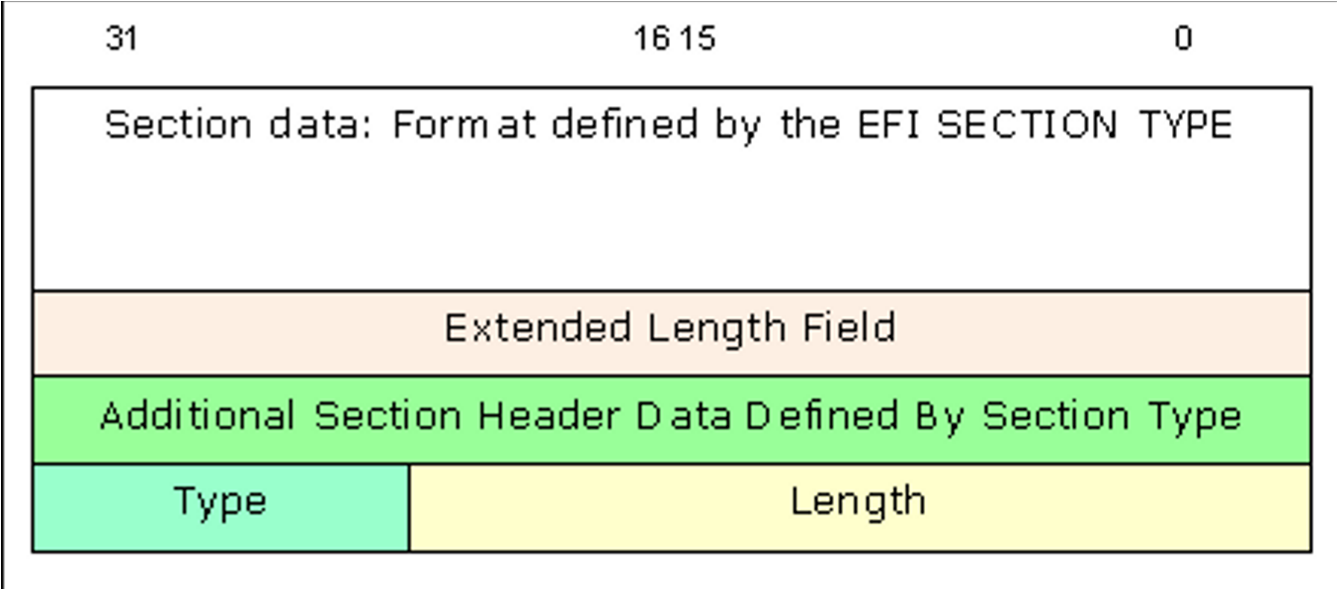
\includegraphics[width=0.7\linewidth]{design/general-efi-section-format-large}
	\caption{General EFI Section Format for large size Sections(greater then 16 MB)}\label{fig:design-general-efi-section-format-large}
\end{figure}


\begin{figure}[h]
	\centering
	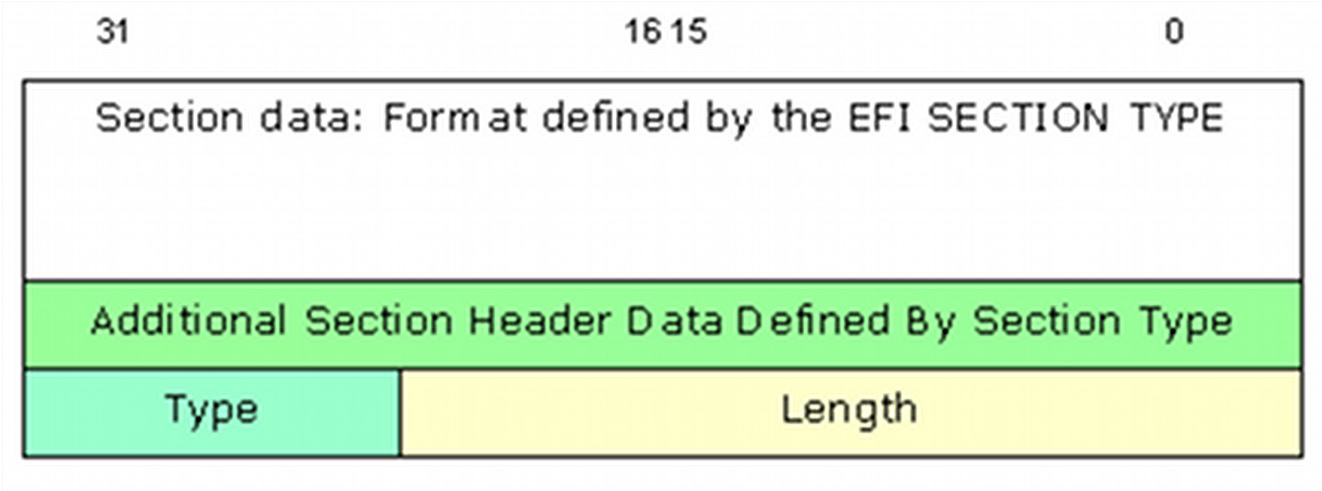
\includegraphics[width=0.7\linewidth]{design/general-efi-section-format}
	\caption{General EFI Section Format (less then 16 MB)}\label{fig:design-general-efi-section-format}
\end{figure}

